%!TEX root = main.tex
\section{Introducción}

El método Monte Carlo es una técnica poderosa y ampliamente utilizada en el transporte de radiación. Su principal ventaja radica en la ausencia de aproximaciones sobre la distribución angular de los flujos de partículas, lo cual asegura una representación fiel incluso en problemas relativamente difíciles, como aquellos con absorbentes fuertes o propagación en vacío.

Un problema de transporte de radiación por Monte Carlo queda esencialmente definido por tres elementos principales:
\begin{itemize}
    \item Geometría: representación del sistema físico a modelar. Incluye los materiales involucrados y las condiciones de contorno.
    \item Fuente: región donde nacen las partículas, con una dada distribución energética, espacial y angular.
    \item Detector (\emph{tally}): resultado a obtener de la simulación, usualmente asociado al nivel de flujo o corriente en una región de interés. El cómputo del valor a reportar se realiza en base a las partículas que llegan al detector.
\end{itemize}

La principal dificultad del método Monte Carlo es el relativamente alto costo computacional requerido para obtener resultados confiables. La confiabilidad de un resultado se mide por su varianza estadística, la cual a su vez se relaciona con la cantidad de partículas utilizadas para calcularlo. Para resolver dicha problemática existen diferentes estrategias conocidas como \emph{técnicas de reducción de varianza}, las cuales buscan favorecer la propagación de la radiación hacia la región de interés, respetando la física del problema.

La herramienta KDSource permite la implementación de una técnica de reducción de varianza, la cual se denominará método KDSource. Los problemas de interés son entonces situaciones en las cuales no es posible alcanzar estadística suficiente en el detector en una única corrida, pues el costo computacional sería demasiado alto. Desde luego, siempre es posible determinar una superficie más cercana a la fuente en la cual sí es posible alcanzar buena estadística. Dicha situación se esquematiza en la Figura \ref{fig:esq_mc}, y es en la que se basa la aplicación del método KDSource.

Continuando con el ejemplo de la Figura \ref{fig:esq_mc}, el método KDSource consiste en registrar las partículas que atraviesan la superficie S1, obteniendo una lista de partículas (energía, posición, dirección) con estadística suficiente. Luego se utiliza dicha lista, también llamada lista de \emph{tracks}, para estimar la distribución de corriente en S1, y se utiliza dicha distribución estimada como fuente en una nueva simulación. La cantidad de partículas producidas en esta segunda etapa puede superar el tamaño de la lista original, mejorando la estadística en la región del detector y reduciendo la varianza del resultado. Todo este proceso se muestra en la Figura \ref{fig:esq_rv}. 

\begin{figure}[h!]
    \centering
    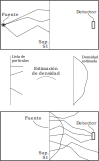
\includegraphics[width=.8\textwidth]{figs/esquema_simul.pdf}
    \caption{Esquema básico de una simulación por Monte Carlo. La superficie S1 permite la implementación de la técnica de reducción de varianza con la herramienta KDSource.}
    \label{fig:esq_mc}
\end{figure}

\begin{figure}[htbp!]
    \centering
    \includegraphics[width=.7\textwidth]{figs/esquema_redvar.pdf}
    \caption{Esquema de la implementación del método KDSource. Se utiliza una lista de partículas registrada en una superficie intermedia para estimar su distribución, y utilizar esta última como fuente en una segunda simulación.}
    \label{fig:esq_rv}
\end{figure}


\subsection{\emph{Kernel Density Estimation}}
\label{subsec:kde}

El método empleado para la estimación de densidad es \emph{Kernel Density Estimation} (KDE). El mismo se basa en la siguiente expresión para la densidad estimada:

\begin{equation}
    \tilde{p}(x) = \frac{1}{N} \sum_{i=1}^N \frac{1}{|H|} K(H^{-1} (x-x^{(i)}))
    \label{eq:KDE}
\end{equation}
Donde:
\begin{itemize}
    \item $X = \{x^{(i)} \in \mathbb{R}^D\}_{1\leq i \leq N}$ es el conjunto de muestras que representa la lista de partículas.
    \item $\tilde{p}(x)$ es la densidad estimada en función del vector $x=(x_1,...,x_D)$.
    \item $K$ es el \emph{kernel} del método, que en KDSource es la distribución normal (\emph{gaussiana}).
    \item $H$ es el ancho de banda (\emph{bandwidth}). En el caso más general considerado en KDSource $H=H^{(i)}=(h_1^{(i)},...,h_D^{(i)})$ es un vector, el cual puede ser diferente para cada partícula. Cuando $H^{(i)}$ es diferente para cada partícula se dice que el método KDE es adaptativo.
\end{itemize}

Considerando el \emph{kernel} \emph{gaussiano} y el ancho de banda vector la expresión resulta:
\begin{equation}
    \label{eq:KDE-gauss}
    \tilde{p}(x) = \frac{1}{N (2\pi)^{D/2}} \sum_{i=1}^N \frac{1}{\prod_j h_j^{(i)}} exp\left(-\frac{1}{2} \sum_j \left(\frac{x_1-x_1^{(i)}}{h_1^{(i)}}\right)^2\right)
\end{equation}

El muestreo consiste en obtener nuevas muestras $\tilde{X} = \{\tilde{x}^{(i)} \in \mathbb{R}^D\}_{1\leq i \leq M}$ respetando la densidad estimada en \ref{eq:KDE}. Para el método KDE, la misma se realiza con el siguiente algoritmo:
\begin{itemize}
    \item Se toma un $x^{(i)} \in X$.
    \item Se obtiene la nueva muestra como $x = x^{(i)} + \Delta$, siendo $\Delta$ una perturbación aleatoria con la distribución del \emph{kernel} (\emph{gaussiana}) y los anchos de banda correspondientes a $x^{(i)}$.
\end{itemize}
Al repetir el muestreo, los $x^{(i)}$ se van tomando en orden tal como están en la lista de partículas. Cuando se llega al final, se vuelve al principio.

El ancho de banda es el parámetro más importante del método KDE. Para que la estimación de densidad tenga el mínimo error posible, los anchos de banda deben ser optimizados. Para ello KDSource incluye tres métodos:
\begin{itemize}
    \item Regla de Silverman: Estima el ancho de banda óptimo únicamente en base a la cantidad de partículas en la lista, su dimensionalidad, y la desviación estándar $\sigma$ de cada variable. Es un método simple y rápido, aunque puede resultar en sobre-suavizado. Su fórmula es la siguiente:
    \begin{equation}
        h_{j,silv} = \left(\frac{4}{2+D}\right)^{\frac{1}{4+D}} N^{-\frac{1}{4+D}}
    \end{equation}  
    \item K Vecinos Más Cercanos (KNN): Calcula el ancho de banda para cada variable como la distancia al K-ésimo vecino más cercano, dentro de la lista de partículas, donde K es un parámetro fijado por el usuario. Es una técnica relativamente sencilla y rápida para obtener un ancho de banda variable (KDE adaptativo). 
    \item Validación Cruzada de Máxima Probabilidad (MLCV): Se basa en la maximización de la log-probabilidad media por validación cruzada, la cual funciona como factor de mérito de la estimación de densidad. Para ello se divide $X$ en dos conjuntos $X_{train}$ y $X_{test}$, y se calcula el factor de mérito como:
    \begin{equation}
        FM = \frac{1}{N_{test}} \sum_{X_{test}} \tilde{p}_{train}(x^{(i)}) 
    \end{equation}
    Donde $\tilde{p}_{train}$ es el modelo KDE construido con $X_{train}$.

    Se construye una grilla de anchos de banda partiendo de una semilla y una grilla de factores. Para cada ancho de banda se calcula el factor de mérito, y se toma el ancho de banda que lo maximiza. Es un método costoso computacionalmente, pero robusto ante diferentes distribuciones. Se obtiene la máxima optimización cuando se utiliza como semilla un ancho de banda obtenido por KNN.
\end{itemize}

El carácter multidimensional del ancho de banda, es decir que $h_j^{(i)}$ sea diferente para cada variable $j$, puede simplificarse a un caso unidimensional, donde $h_1^{(i)}=...=h_D^{(i)}$, mediante la normalización de datos. Usualmente, los anchos de banda para cada dimensión se toman como proporcionales a la desviación estándar de cada variable, es decir:
\begin{equation}
    h_j^{(i)} = h^{(i)} \sigma_j
\end{equation}
Introduciendo esta expresión en \ref{eq:KDE-gauss} se obtiene:
\begin{equation}
    \label{eq:DN}
    \tilde{p}(x) = \frac{1}{N (2\pi)^{D/2}} \sum_{i=1}^N \frac{1}{(h^{(i)})^D\prod_j \sigma_j} exp\left(-\frac{1}{2} \sum_j \left(\frac{x_1-x_1^{(i)}}{h^{(i)}\sigma_j}\right)^2\right)
    = \frac{1}{\prod_j \sigma_j} \tilde{p}_n(x_n)
\end{equation}
Donde $x_n=(\frac{x_1}{\sigma_1},...,\frac{x_D}{\sigma_D})$ es el vector normalizado, y $\tilde{p}_n$ es el modelo KDE construido con el conjunto de vectores normalizados, con anchos de banda $h^{(i)}$ unidimensionales.

La técnica consiste entonces en normalizar el conjunto $X$ de datos, empleando los $\sigma_j$ u otros factores de escaleo considerados apropiados, luego construir el modelo KDE normalizado $\tilde{p}_n(x_n)$, y finalmente obtener el modelo general de la ecuación \ref{eq:DN}. Los métodos de optimización de ancho de banda se aplican sobre el modelo normalizado.


\subsection[KDE en simulaciones Monte Carlo: ¿Cuándo y por qué es útil el método KDE?]{KDE en simulaciones Monte Carlo:\\¿Cuándo y por qué es útil el método KDE?}
\label{ssec:KDE-MC}

Considérese una simulación general por Monte Carlo con un único \emph{tally} $R$ y una fuente con distribución $S(x)$. En esta Subsección se analizará el impacto del error sistemático introducido por una fuente KDE sobre el valor de $R$, comparado con el muestreo directo de la lista de partículas, lo cual se denominará fuente de \emph{tracks}. Se utilizará para ello la propiedad de las distribuciones de Poisson según la cual, al contar en un \emph{tally} $n$ partículas, se tiene un error estadístico de $\sqrt{n}$.

Desde el punto de vista de la función importancia, también llamada flujo adjunto o función de Green \cite{AF}, el valor del \emph{tally} puede expresarse como:
\begin{equation}
    \label{eq:R}
    R = \int I(x) S(x) dx \approx I_0 \int_{\Omega} S(x) dx
\end{equation}
Donde $I$ es la función importancia, y la integración es sobre todo el espacio de fases. En la expresión aproximada se toma $I(x)$ como $I_0$ para $x \in \Omega$, y 0 afuera.

La fuente de \emph{tracks} puede expresarse como una suma de deltas de Dirac:
\begin{equation}
    S_t(x) = \frac{1}{N} \sum_i \delta\left(x-x^{(i)}\right)
\end{equation}

El valor del \emph{tally} resulta entonces:
\begin{equation}
    \label{eq:Rt}
    R_t = \frac{1}{N} \sum_i I(x^{(i)}) \approx \frac{n_{\Omega} I_0}{N}
\end{equation}
Donde $n_{\Omega}$ es la cantidad de partículas en la lista dentro de la región $\Omega$.

Por lo tanto, el error del \emph{tally} asociado a la fuente, en este caso, se puede estimar como:
\begin{equation}
    \frac{\Delta R_t^{sist}}{R_t} = \frac{1}{\sqrt{n_{\Omega}}}
\end{equation}

Para la fuente KDE, por simplicidad, se supondrá un ancho de banda único $h$, ya optimizado. Para la estimación de $R$ con dicha fuente se distinguirán dos situaciones:
\begin{itemize}
    \item $\mu(\Omega) >> h^D$
    \item $\mu(\Omega) << h^D$
\end{itemize}
Donde $\mu(\Omega)$ es la medida de la región $\Omega$.

En el primer caso, al ser el ancho de banda mucho menor a la longitud característica de $\Omega$, el resultado en el \emph{tally} resultará muy similar al caso con fuente de \emph{tracks}. También será similar el error asociado a la fuente, salvo por un \emph{bias} dependiente del valor medio de la pendiente de la distribución de fuente en la frontera de $\Omega$.

En este caso se puede concluir que el método KDE no resulta de gran utilidad, ya que no mejora el error del \emph{tally} asociado a la fuente. Resulta más apropiado utilizar la fuente de \emph{tracks}, si es necesario muestreando varias veces cada partícula en la lista, para reducir el error estadístico de la simulación.

En el segundo caso, al ser el ancho de banda mucho mayor a la longitud característica de $\Omega$, se puede suponer a $S_{KDE}(x)$ como lineal dentro de $\Omega$, y aproximar $R$ como:
\begin{equation}
    R_{KDE} = I_0 \mu(\Omega) S_{KDE}(x_0)
\end{equation}
Donde $S_{KDE}$ es la distribución de la fuente KDE, y $x_0$ es un vector de fase dentro de $\Omega$.

El error de $R$ asociado a la fuente, en este caso, se obtiene directamente del error puntual del método KDE. El mismo se compone de un error estadístico, que depende de la cantidad de partículas usadas en la estimación, y un \emph{bias} por el suavizado \cite{NP}.
\begin{equation}
    \frac{\Delta R_{KDE}^{sist}}{R_{KDE}} = \frac{\sqrt{r}}{\sqrt{n_h}} + bias(x_0)
\end{equation}
Donde $n_h$ es la cantidad de partículas dentro de una hiper-esfera de radio $h$ centrada en $x_0$, y $r$ es la denominada rugosidad del \emph{kernel}, que vale $1/2\sqrt{\pi}$ para el \emph{kernel} \emph{gaussiano}. Para otros \emph{kernels} siempre es del orden de 1.

Es en este caso en el que el método KDE puede resultar útil, reduciendo el error en el \emph{tally} asociado a la fuente. Debido a que $\mu(\Omega) << h^D$, se tiene que $n_{\Omega} << n_h$, y por lo tanto $1/\sqrt{n_{\Omega}} >> 1/\sqrt{n_h}$. Es decir que el método KDE reduce significativamente el error de $R$ asociado al error estadístico de la fuente, aunque a costa de un error adicional asociado al \emph{bias}. Si bien no es posible asegurar de forma general el resultado de dicho balance, es de esperar que, gracias a la optimización del ancho de banda, una mejora sea probable.

En conclusión, las situaciones en la que el método KDE resulta más útil son aquellas en las que la región de la fuente que afecta el \emph{tally} es pequeña, con pocas partículas en su interior, y en particular con distancias características menores al ancho de banda optimizado. Al haber pocas partículas en la región de fuente ``observada'' por el \emph{tally}, el error asociado a una fuente de \emph{tracks} es grande, y el suavizado que realiza el método KDE, teniendo en cuenta un mayor número de partículas, resulta beneficioso. Estas situaciones pueden relacionarse con problemas de propagación en vacío, donde existen pocos caminos por los cuales las partículas pueden llegar de la fuente a la región de interés, en contraposición con los problemas de moderación.

La herramienta KDSource, a pesar de estar esencialmente orientada a fuentes KDE, también permite implementar fuentes de \emph{tracks}, y en ambos casos facilita el acople entre códigos Monte Carlo.
